%/!\ /!\ 
%
% PLEASE DO NOT EDIT THIS IF YOU CAME HERE BY MISTAKE !!!!
%

% RTFMN : https://tobi.oetiker.ch/lshort/lshort.pdf

\documentclass{article}
\usepackage{xspace}
\usepackage[utf8]{inputenc}
\usepackage[T1]{fontenc}
\usepackage[english]{babel}
\usepackage{amsmath}
\usepackage{amsthm}
\usepackage{graphicx}
\usepackage{url}
\usepackage{amssymb}
\usepackage{mathrsfs}
\usepackage{amsfonts}
\usepackage{multicol}
\usepackage{stmaryrd}
\usepackage{tikz, pgf}
\usetikzlibrary{arrows,intersections}
\usetikzlibrary{automata,positioning} %pour els machines de Turing
\usepackage{libertine}
\usepackage[a4paper,left=2cm,right=2cm,top=2cm,bottom=2cm]{geometry}
\usepackage{dsfont}


\usepackage[linktocpage]{hyperref}

\setlength{\hoffset}{-18pt}         
\setlength{\oddsidemargin}{15pt} % Marge gauche sur pages impaires
\setlength{\evensidemargin}{15pt} % Marge gauche sur pages paires
\setlength{\marginparwidth}{0pt} % Largeur de note dans la marge
\setlength{\textwidth}{481pt} % Largeur de la zone de texte 
\setlength{\marginparsep}{7pt} % Séparation de la marge
\setlength{\topmargin}{0pt} % Pas de marge en haut
\setlength{\headheight}{13pt} % Haut de page
\setlength{\headsep}{10pt} % Entre le haut de page et le texte
\setlength{\footskip}{50pt} % Bas de page + séparation
\setlength{\textheight}{600pt} % Hauteur de la zone de texte 

%\setlength{\hoffset}{-18pt}         
%\setlength{\oddsidemargin}{15pt} % Marge gauche sur pages impaires
%\setlength{\evensidemargin}{15pt} % Marge gauche sur pages paires
%\setlength{\marginparwidth}{0pt} % Largeur de note dans la marge
%\setlength{\textwidth}{481pt} % Largeur de la zone de texte 
%\setlength{\marginparsep}{7pt} % Séparation de la marge
%\setlength{\topmargin}{0pt} % Pas de marge en haut
%\setlength{\headheight}{8pt} % Haut de page
%\setlength{\headsep}{0pt} % Entre le haut de page et le texte
%\setlength{\footskip}{15pt} % Bas de page + séparation
%\setlength{\textheight}{700pt} % Hauteur de la zone de texte 

%\newcommand{\ket}[1]{\ensuremath{|#1\rangle}\xspace}
%\newcommand{\bra}[1]{\ensuremath{\langle #1|}\xspace}

\newtheorem{thm}{Theorem}[section]
\newtheorem{prop}[thm]{Proposition}
\newtheorem{lem}[thm]{Lemma}
\newtheorem{cor}[thm]{Corollary}
\newtheorem{defi}[thm]{Definition}

\newcommand{\Thm}[3]{\begin{thm}[#1]\label{#2}#3\end{thm}}
\newcommand{\Ex}[3]{\begin{ex}[#1]\label{#2}#3\end{ex}}
\newcommand{\Def}[3]{\begin{defi}[#1]\label{#2}#3\end{defi}}
\newcommand{\Lem}[3]{\begin{lem}[#1]\label{#2}#3\end{lem}}
\newcommand{\Cor}[3]{\begin{cor}[#1]\label{#2}#3\end{cor}}
\newcommand{\Prop}[3]{\begin{prop}[#1]\label{#2}#3\end{prop}}

\newcommand{\hsp}{\hspace{20pt}}
\newcommand{\HRule}{\rule{\linewidth}{0.5mm}}
\newcommand{\R}{\mathbb{R}}
\newcommand{\N}{\mathbb{N}}
\newcommand{\K}{\mathbb{K}}
\newcommand{\Q}{\mathbb{Q}}
\newcommand{\C}{\mathcal{C}}
\newcommand{\brakets}[1]{\langle#1\rangle}

\newcommand{\ind}[1]{\mathds{1}_{#1}}

\title{Computational Complexity : HW 1}

\author{Quentin Guilmant}
\date{\today}

\begin{document}
\maketitle

Let $\Sigma$ be a finite set and $Pal\equiv\{x\in\Sigma^*|x=\bar{x}\}$.\\
Let $\Sigma'=\Sigma\cup\{\vartriangleright,\square\}$.

In the following the notation $(a,b)|(c,d),(x,y)$ with $a,b,c,d$ some characters and $x,y\in\{L,S,R\}$ some directions, states for we read $a$ on first tape, $b$ on second tape, then we write $c$ on the first and $d$ on the second, then we move according to the direction $x$ on first tape and according $y$ on the second one.

We assume that the first tape is for the input. At the beginning we have $\vartriangleright x\square...$ on the first tape with $x\in\Sigma^*$ the input word and on the other tapes $\vartriangleright\square...$. 

For any Turing Machine $\mathcal{M}$ we denotes $\mathcal{L}(\mathcal{M})$ the language recognized by the machine.

\section{A Turing Machine that recognizes $Pal$ in linear time with two tapes}
Let us consider the following Turing machine.

\begin{tikzpicture}[shorten >=1pt,node distance=4cm,on grid,auto]
	\node[state,initial] (start) {$q_{start}$};
	\node[state] (1) [right=of start] {$q_1$};
	\node[state] (2) [right=of 1] {$q_{compare}$};
	\node[state] (a) [below=of 1] {$q_{accept}$};
	\node[state] (r) [below=of 2] {$q_{reject}$};
	
	\path[->]
		(start)	edge [loop below] 	node {$\begin{array}{c}
		(\vartriangleright,\vartriangleright)|(\vartriangleright,\vartriangleright),(R,R)\\
		\forall a\in\Sigma,(a,\square)|(a,a),(R,R)
		\end{array}$} (start)
		(start)	edge 				node {$(\square,\square)|(\square,\square),(L,L)$} (1)
		(1)		edge [loop below]	node {$\forall a,b\in\Sigma,(a,b)|(a,b),(L,S)$} (1)
		(1)		edge 				node {$(\vartriangleright,b)|(\vartriangleright,b),(R,S)$} (2)
		(2)		edge [loop right]	node {$\forall a\in\Sigma (a,a)|(a,a)(R,L)$} (2)
		(2)		edge				node {$\forall a,b\in\Sigma,a\neq b,(a,b)|(a,b),(S,S)$} (r)
		(2)		edge				node [left] {$(\square,\vartriangleright)|(\square,\vartriangleright),(S,S)$} (a)
		;
\end{tikzpicture}

This Turing machine works on the alphabet $\Sigma'$.

\Lem{Copy}{lem:copy}{For every input $x\in\Sigma^*$, at the first time state $q_1$ is reached, the tapes are on the same configuration: $\vartriangleright x\square$ and both tapes are pointing to the last character of $x$, and this time is linear in $n=|x|$. }

\begin{proof}
Let $x=x_1...x_n$ the input. In the following $x_{n+1}=\square$ and $x_0=\vartriangleright$. The positions of the state start form $0$ ($\vartriangleright$).  Let us consider the following property:\\
$(H_k)$: after $k$ transitions, the machine is still in state $q_{start}$ and the tapes are on the following configuration: $\vartriangleright x\square$ for the first one and $\vartriangleright x_1... x_{k-1}\square$ for the second one. Both tapes are pointing to position $k$.

\begin{itemize}
\item $(H_0)$ is satisfied as it is the definition of the initial configuration.
\item The first transition is on $(\vartriangleright,\vartriangleright)$ then we just go to the right one both tapes. $(H_1)$ is true.
\item Suppose $(H_k)$ is true for some $1\leq k <n+1$. Then the current state is still $q_{start}$ and we read  $(x_k,\square)$ according to $(H_k)$. $k<n+1$ then $x_k\neq\square$ and we loop on $q_start$ and we write $x_k$ in position $k$ on the second tape and move right on both tapes. $(H_{k+1})$ is true.
\end{itemize}

Then $(H_{n+1})$ is true. Then the the transition $n+2$ we read $(\square,\square)$ and go to state $q_1$ and move left on both tape. Then are pointing to position $n$. That concludes the proof.\end{proof}

\Lem{Initialization}{lem:init}{For every input $x\in\Sigma^*$, at the first time state $q_{compare}$ is reached, the tapes are on the same configuration: $\vartriangleright x\square$. The first tapes is pointing to position $1$ and the second one to position $n$. Moreover, this time is linear in $n=|x|$. } 

\begin{proof}
Using lemma \ref{lem:copy} we know that when we arrive in $q_1$ we have the correct tapes, the second one pointing to the correct place but not the first one. All the transition going from $q_1$ are going to $q_1$ or $q_compare$. All the transition do not change what is written on the tapes and the position of the second tape. One can easily prove by recurrence the following property:\\
$(H_k^2)$: after $t_1+k$  transitions, the tapes are in the same configuration, $\vartriangleright x\square$, the first one is pointing to the position $n-k$ and the second one to the position $n$.\\
Where $t_1$ is the number of transitions until the machine reaches $q_1$ for the first time. One must prove it for $0\leq k\leq n$. It is basically the same proof as previously.

The last transition from $q_1$ to $q_{compare}$ concludes.
\end{proof}

\Prop{The machine recognizes $Pal$}{prop:palLinear}{Let $\mathcal{M}$ be the given Turing Machine, $\mathcal{L}(\mathcal{M})=Pal$. This machine halts in linear time}

\begin{proof}
Let $x\in\Sigma^*$. We use lemma \ref{lem:init} to get the initialization of the computation. Let $t_2$ the number of transition until we reach state $q_{compare}$ for the first time. Thanks to the previous lemmas, it is linear in $n$. Let $y$ the longest word such that $\exists z,x=yz\bar{y}$. Let $y=y_1...y_m$. We still consider $z$ associated to $y$. Consider the  following property:\\
$(H_k^3)$:after $t_2+k$ transitions, the state is still $q_{compare}$, the tapes do not have changed and are pointing respectively to positions $1+k$ and $n-k$.

We have to prove it for $0\leq k\leq m$. 
\begin{itemize}
\item $(H_0^3)$ is the definition of the first time we reach $q_{compare}$ and then is direct implication from lemma \ref{lem:init}.
\item Suppose $(H_k^3)$ is true for some $0\leq k <m$. Because $k<m$ the two tapes are respectively pointing to a cell containing $x_{k+1}=y_{k+1}=x_{n-k}\notin\{\vartriangleright,\square\}$. Then we read $(y_{k+1},y_{k+1})$ and the only transition possible is going again to $q_{compare}$, do not change what is written on the tapes the tapes respectively move right and left what proves $(H_{k+1}^3)$.
\end{itemize}
Then $(H_m^3)$ is true.

\begin{itemize}
\item If $x\in Pal$, then $|z|\in\{0,1\}$ (it is in fact an equivalence).
\begin{itemize}
\item if $|z|=0$. Then $n=2m$, the first tape is pointing to $x_{m+1}=\bar{y}_{1}=y_{m}$ and the second one is pointing to $x_{n-m}=x_{m}=y_{m}$. Consider the  following property:\\
$(H_k^4)$:after $t_2+m+k$ transitions, the state is still $q_{compare}$, the tapes do not have changed and are pointing respectively to positions $1+m+k$ and $n-m-k$.

We have to prove it for $0\leq k\leq m$.
\begin{itemize}
\item $(H_0^4)$ is the same property as $(H_m^3)$ which has already been proved.
\item Suppose $(H_k^4)$ is true for some $0\leq k <m$. Because $k<m$ the two tapes are respectively pointing to a cell containing $x_{m+k+1}=\bar{y}_{k+1}=y_{m-k}=x_{n-m-k}\notin\{\vartriangleright,\square\}$. Then we read $(y_{m-k},y_{m-k})$ and the only transition possible is going again to $q_{compare}$, do not change what is written on the tapes the tapes respectively move right and left what proves $(H_{k+1}^4)$.
\end{itemize}

Then $(H_m^4)$ is true and the tape are pointing respectively to $\square$ and $\vartriangleright$. The only transition possible goes to $q_{accept}$ what conclude the proof.
\item otherwise $|z|=1$ and $n=2m+1$. With $(H_m^3)$ we have that tapes are pointing to the same cell, the position $m+1=n-m$ containing $z\notin\{\vartriangleright,\square\}$. The only transition possible goes to $q_{compare}$, do not change what os written on the tapes and are now respectively pointing to position $m+2$ and $n-m-$. Consider the following property:\\ 
$(H_k^5)$:after $t_2+m+1+k$ transitions, the state is still $q_{compare}$, the tapes do not have changed and are pointing respectively to positions $2+m+k$ and $n-m-1-k$.

We have to prove it for $0\leq k\leq m$.
\begin{itemize}
\item $(H_0^5)$ as been proved just before the definition of the property.
\item Suppose $(H_k^5)$ is true for some $0\leq k <m$. Because $k<m$ the two tapes are respectively pointing to a cell containing $x_{m+k+2}=\bar{y}_{k+1}=y_{m-k}=x_{n-m-1-k}\notin\{\vartriangleright,\square\}$. Then we read $(y_{m-k},y_{m-k})$ and the only transition possible is going again to $q_{compare}$, do not change what is written on the tapes the tapes respectively move right and left what proves $(H_{k+1}^5)$.
\end{itemize}
Then $(H_m^5)$ is true and the tape are pointing respectively to $\square$ and $\vartriangleright$. The only transition possible goes to $q_{accept}$ what conclude the proof.
\end{itemize}
\item If $x\notin Pal$. Then $|z|\geq 2$. Using $(H_m^3)$ the tapes are pointing to respectively $z_1\notin\{\vartriangleright,\square\}$ and $z_{|z|}\notin\{\vartriangleright,\square\}$. We have $z_1\neq z_{|z|}$, otherwise it makes a contradiction with the fact that $y$ is the longest word such that $x=yz\bar{y}$. Then, the only transition goes to $q_{reject}$ what concludes the proof.
\end{itemize}

Know in all cases the halting time is $t_2+l(m)$ with $t_2$ linear and $l$ an increasing polynomial of degree $1$. Then, since $m\leq n$ the halting time is linear in $n$. 
\end{proof}

\section{A Turing Machine that recognizes $Pal$ in quadratic time with one tape}
We know work on the alphabet $\Gamma=\Sigma'\cup\{X\}$. We also denote $\Sigma=\{a_1,...a_p\}$. The following Turing machine, let us call is $\mathcal{M_q}$ recognizes $Pal$ in quadratic time and have only one tape. The $X$ will stand for «already managed character».

\begin{center}
\begin{tikzpicture}[shorten >=1pt,node distance=3cm,on grid,auto]
	\node [state,initial]	(start)						{$q_{start}$};
	\node [state]			(a)		[right=of start]	{$q_{accept}$}; 
	\node [state]			(1)		[below=of start]	{$q_{a_1}$};
	\node [state]			(k)		[right=of 1]		{$...$};
	\node [state]			(p)		[right=of k]		{$q_{a_p}$};
	\node [state]			(1f)	[below=of 1]		{$q_{a_1,f}$};
	\node [state]			(pf)	[below=of p]		{$q_{a_p,f}$};
	\node [state]			(r)		[right=of 1f]		{$q_{reject}$};
	\node [state]			(rinit)	[below=of r]			{$q_{re-init}$};
	\node [state]			(flag)	[left=of 1f]		{$q_{flag}$};
	
	\path[->]
		(start)	edge	[loop above]		node {$\vartriangleright|\vartriangleright,R$} (start)
		(start) edge						node {$\begin{array}{c}X|X,S\\ \square|\square,S\end{array}$} (a)
		(start) edge						node [right] {$a_1|a_1,R$} (1)
		(start) edge						node [right=0.005] {$a_k|a_k,R$} (k)
		(start) edge						node {$a_p|a_p,R$} (p)
		(1)		edge						node {$\begin{array}{c}X|X,L\\ \square|\square,L\end{array}$} (1f)
		(1)		edge	[loop right]		node {$\begin{array}{c}\forall a\in\Sigma\\ a|a,R\end{array}$} (1)
		(p)		edge						node {$\begin{array}{c}X|X,L\\ \square|\square,L\end{array}$} (pf)
		(p)		edge	[loop right]		node {$\begin{array}{c}\forall a\in\Sigma\\ a|a,R\end{array}$} (p)
		(1f)	edge						node {$\begin{array}{c}\forall a\neq a_1\\ a|X,S\end{array}$} (r)
		(1f)	edge						node {$a_1|X,L$} (rinit)
		(pf)	edge						node [above] {$\begin{array}{c}\forall a\neq a_p\\ a|X,S\end{array}$} (r)
		(pf)	edge						node {$a_p|X,L$} (rinit)
		(rinit)	edge	[loop right]		node {$\forall a\in\Sigma, a|a,L$} (rinit)
		(rinit) edge	[out=180, in=270]	node {$\begin{array}{c}\vartriangleright|\vartriangleright,R\\ X|X,R\end{array}$} (flag)
		(flag)	edge	[out=90, in=225]	node {$\forall a\in\Sigma, a|X,R$} (start)
		
		;
\end{tikzpicture}
\end{center}

\Lem{Special input in $Pal$}{lem:specInput}{For all $x\in Pal$, $n,p\in\N$, on configuration $\vartriangleright X^nxX^p\square...$ and tape pointing to position $n+1$ (i.e. to $x_1$) and machine in state $q_{start}$, the machine halts in state $q_{accept}$.}

\begin{proof}
Let us consider the following property:\\
$(H_k)$: for any $x\in Pal$ such that $|x|=k$, with the previous initial configuration, the computation halts in state $q_{accept}$.

\begin{itemize}
\item $(H_0)$ is true: the computation for the empty word $\varepsilon\in Pal$ is $q_{start}\rightarrow q_{accept}$.
\item $(H_1)$ is true: let us take as input $x=a_m$. We first $a_m$ and go to $q_{a_m}$ and we are now pointing to $\square$ or the first $X$ of $X^p$. So we go to $q_{a_m,f}$ and move left, go back pointing to $a_m$. Then we go to $q_{re-init}$ and move left again pointing to $\vartriangleright$ (if $n=0$) or the last $X$ of $X^n$. Then we go to  $q_{flag}$ and move right pointing to $a_m$. We replace it by $X$ and move right pointing to $\square$ (if $p=0$) or the first $X$ of $X^p$ and going to state $q_{start}$ which finishes the computation going on $q_{accept}$.
\item Suppose $H_{k-1}$ and $H_{k}$ for some $k\geq 1$. Let us take $x=x_1...x_{k+1}$ with $x_1=x_{k+1}=a_m$ for some $m$. Let $y=x_2...x_k$. We first read $a_m$ and go to $q_{a_m}$ and we are now pointing to $x_2$. Then we loop on $q_{a_m}$ and move right until we reach the first $X$ of $X^p$ or $\square$ (if $p=0$). So we go to $q_{a_m,f}$ and move left, go back pointing to $x_{k+1}=a_m$. Then we go to $q_{re-init}$ and move left again pointing to $x_k$, replacing $x_{k+1}$ by an $X$. Then we loop on $q_{re-init}$ until we reach the beginning of the tape or the last $X$ of $X^n$ if any. Then we read is and move right back on $x_1$. We replace it by an $X$ an go to $q_{start}$ and move right and now point on $x_2$. Then the current configuration of the tape is $\vartriangleright X^{n+1}yX^{p+1}\square...$, we are pointing on $y_1=x_2$ and the current state is $q_{start}$. Then using $H_{k-1}$ on $y$ ($y\in Pal$ otherwise $x\notin Pal$) we conclude that the machine halts in $q_{accept}$. $(H_{k+1})$ is true.
\end{itemize}
\end{proof}

\Cor{$Pal\subseteq\mathcal{L}(\mathcal{M}_q)$}{cor:PalSubLMq}{Every $x\in Pal$ is accepted by $\mathcal{M}_q$}
\begin{proof}
Let $x\in Pal$. The first transition is the reading of $\vartriangleright$ that loops on $q_{start}$. Then we reach the initial configuration of lemma \ref{lem:specInput} on $x$ with $n=p=0$. Then we conclude.
\end{proof}

\Lem{Special input not in $Pal$}{lem:specInputnPal}{For all $x\in Pal$, $n,p\in\N$, on configuration $\vartriangleright X^nxX^p\square...$ and tape pointing to position $n+1$ (i.e. to $x_1$) and machine in state $q_{start}$, the machine halts in state $q_{reject}$.}

As the proof is very similar to the previous one we just give a sketch of proof.

\begin{proof}
Let $y$ the longest word such that there is some word $z$ such that $x=yz\bar{y}$. Then the proof is exactly the same as the previous lemma. The only difference is that recurrence is just on the size of this $y$. As $x\notin Pal$ we know that $|z|\geq 2$ and that $z_1\neq z_{|z|}$. For initialization ($|y|=0$) just do the same reasoning to say that the only transition possible form $q_{z_1,f}$ reading $z_{|z|}$ is going to $q_{reject}$.  
\end{proof}

\Cor{$\mathcal{L}(\mathcal{M}_q)\subseteq Pal$}{cor:LMqSubPal}{Every $x\notin Pal$ is rejected by $\mathcal{M}_q$}

\begin{proof}
Let $x\notin Pal$. The first transition is the reading of $\vartriangleright$ that loops on $q_{start}$. Then we reach the initial configuration of lemma \ref{lem:specInputnPal} on $x$ with $n=p=0$. Then we conclude.
\end{proof}

\Prop{Correctness}{prop:correctMq}{$\mathcal{L}(\mathcal{M}_q)=Pal$}

\begin{proof}
Just apply corollaries \ref{cor:PalSubLMq} and \ref{cor:LMqSubPal}. 
\end{proof}

\Prop{Halting time}{prop:timeMq}{$\mathcal{M}_q$ halts in quadratic time.}

\begin{proof}
\begin{itemize}
\item Let $x\in Pal$. Consider each iteration of the proof of lemma \ref{lem:specInput}. Let $T_{Pal,k}$ the number of step needed  to stop the computation on input an $x\in Pal$ such that $|x|=k$. We saw that $T_{Pal,0}=3$, $T_{Pal,1}=7$. Then $T_{Pal,k+2}=T_{Pal,k}+1+k+1+1+(k-1)+1+1=T_{Pal,k}+2k+4$ by following the proof. Let $u_k=T_{Pal,2k+1}$. Then $u_0=7$ and $u_{k+1}=u_{k}+4(k+1)$. Then $u_k=7+4\frac{k(k+1)}{2}=7+2k(k+1)$. Let $v_k=T_{Pal,2k}$. Then $v_0=3$ and $v_{k+1}=v_{k}+4(k+1)$. Then, as well as $u_k$, $v_k=3+4\frac{k(k+1)}{2}=3+2k(k+1)$. Then $T_{Pal,k}\leq 7+2\lfloor k\rfloor(\lfloor k\rfloor+1)\leq 7 + 2k(k+1)$, which quadratic in $k$.
\item Let $x\notin Pal$. Consider each iteration of the proof of lemma \ref{lem:specInputnPal}. Let $T_{\overline{Pal},k,m}$ the number of step needed to stop the computation on input an $x\in Pal$ such that $|x|=k$ and such that the associated $y$ has length $m$. We saw that $T_{\overline{Pal},k,0}=1+1+k+1+1=k+4$. Then $T_{\overline{Pal},k+2,m+1}=T_{\overline{Pal},k,m}+1+k+1+1+(k-1)+1+1=T_{\overline{Pal},k,m}+2(k+2)$ by following the proof. Let $u_{k,m}=T_{\overline{Pal},k,m}$ with $m\leq\frac{k}{2}$. Then $u_{k,m}=u_{(k-2m),0}+\sum_{i=k-2m+2,step=2}^{k}2(i+2)$ which is still quadratic in $k$.
\end{itemize}
In all cases the machine halts in quadratic time, what concludes the proof.
\end{proof}

\section{Optimality of the previous simulation.}
Let us define $C_i(x)$ thee sequence of states $(q_j)_{j\in\llbracket1;j_i\rrbracket}$ such that $q_1$ is the state we reach when the head of the tape points to cell $i+1$ for the first time, $q_2$ is the state when for the first time after $q_1$ the head is pointing on cell $i$, and so on.

Let $Pal_n=\{x0^{2n}\bar{x}|x\in\Sigma^n\}$.

We will consider a $1$-tape Turing Machine $\mathcal{M}$ that recognizes $Pal$ and halts in time $T(n)$.
\subsection{Equalities between crossing sequences and equality between word.}
\Lem{Building recognized word from others}{lem:buildRecog}{Let $x,y\in\mathcal{L}(\mathcal{M})$, such that $C_i(x)=C_i(y)$. Let $x_{1..i}$ be the prefix of length $i$ of $x$. We the same notation we have $x_{1...i}y_{i+1...|y|}\in\mathcal{L}(\mathcal{M})$.}
\begin{proof}
The crossing states are the same. Let $q_1^x,...,q_{n_x}^x$ be the sequence of states of the computation of $\mathcal{M}$ on input $x$, and $q_1^y,...,q_{n_y}^y$ the one on input $y$. Let $q_1,...,q_k=C_i(x)=C_i(y)$. We consider $\forall i,q_i=q_{j_i^x}^x=q_{j_i^y}^y$, respect to the order.
\begin{itemize}
\item if $k$ is even, $k=2k'$. Then \[q_1^x,...q_{j_1^x}^x,q_{j_1^y+1}^y,...q_{j_2^y}^y,q_{j_2^x+1}^x,...,q_{j_{2p+1}^x}^x,q_{j_{2p+1}^y+1}^y,...,q_{j_{2(p+1)}^y}^y,q_{j_{2(p+1)}^x+1}^x,...,q_{j_{2k'}^y}^y,q_{j_{2k'}^x+1}^x,...q_{n_x}^x\] is the sequence of state on input $x_{1...i}y_{i+1...|y|}$. Then is finishes in an (the) accepting state.
\item if $k$ is odd, $k=2k'+1$. Then \[q_1^x,...q_{j_1^x}^x,q_{j_1^y+1}^y,...q_{j_2^y}^y,q_{j_2^x+1}^x,...,q_{j_{2p+1}^x}^x,q_{j_{2p+1}^y+1}^y,...,q_{j_{2(p+1)}^y}^y,q_{j_{2(p+1)}^x+1}^x,...,q_{j_{2k'+1}^x}^x,q_{j_{2k'+1}^y+1}^y,...q_{n_y}^y\] is the sequence of state on input $x_{1...i}y_{i+1...|y|}$. Then is finishes in an (the) accepting state.
\end{itemize}
\end{proof}
\Prop{}{prop:3.1}{Let $x,y\in Pal_n$. $\exists x',y'\in\Sigma^n,x=x'0^{2n}\overline{x'}\wedge y=y'0^{2n}\overline{y'}$. Let us suppose the machine is deterministic and that $\exists i\in\llbracket n+1,3n-1\rrbracket, C_i(x) = C_i(y)$. Then $x=y$.}
\begin{proof}
Let us take $z=x'0^{2n}\overline{y'}$. Just apply lemma \ref{lem:buildRecog} on $x,y,z,i$ to get that $z\in Pal$. Then we get that $\overline{x'}=\overline{y'}$. Then $x'=y'$ and $x=y$.
\end{proof}

\subsection{Upper bound on $|C_i(y)|$}
\Prop{}{prop:upBound}{Let $y\in Pal_n$. $\exists i\in\llbracket n+1,3n-1\rrbracket, |C_i(y)|\leq\frac{T(4n)}{2n-1}$.}
\begin{proof}
Suppose $\forall i\in\llbracket n+1,3n-1\rrbracket, |C_i(y)|>\frac{T(4n)}{2n-1}$. Then $\sum_{i=n+1}^{3n-1}|C_i(y)|>(2n-1)\frac{T(4n)}{2n-1}=T(4n)$. $y\in Pal_n\subseteq Pal$ and $|y|=4n$, then $\mathcal{M}$ halts on input $y$ in time lower than $T(4n)$. 

Let $q_1,...,q_{n_y}$, the sequence of states corresponding to the computation on input $y$. We can see $C_i(y)$ as a subset of $\llbracket1;n_x\rrbracket$ such that $j\in C_i(y)\Leftrightarrow \text{The transition $q_{j-1}\rightarrow q_j$ crosses the edge between cells $i$ and $i+1$}$. Then if $i\neq i'$, $C_i(y)\cap C_{i'}(y) = \emptyset$. Then $n_y\geq\sum_{i=n+1}^{3n-1}|C_i(y)|>(2n-1)\frac{T(4n)}{2n-1}=T(4n)$. However $n_y\leq T(4n)$ because $\mathcal{M}$ halts in time $T(4n)$. Then we get a contradiction and then the result.
\end{proof}

\subsection{Conclusion}
Let us define for any $c$ $E_c\equiv\{n|T(n)\geq cn^2 + O(n)\}$.
\Prop{Main result}{prop:main}{$\exists c, |E_c|=\infty$}
\begin{proof}
Consider the following function $f:\begin{array}{c c c}
Pal_n & \rightarrow & Q^*\\
y & \mapsto & C_{n+1}(y)
\end{array}$. Using proposition \ref{prop:3.1}, the function $f$ is injective and $|f(y)|\leq\frac{T(4n)}{2n-1}$ using proposition \ref{prop:upBound}. Then:
\[\begin{array}{r c l}
|\Sigma|^n & \leq & |Q|^{\frac{T(4n)}{2n-1}}\\
n\log_{|Q|}(|\Sigma|) & \leq & \frac{T(4n)}{2n-1} \\
T(4n) & \geq & 2\log_{|Q|}(|\Sigma|)n^2-\log_{|Q|}(|\Sigma|)n
\end{array}\]
Then $4\N\subseteq E_{2\log_{|Q|}(|\Sigma|)}$, what concludes the proof.
\end{proof}
\end{document}
